\documentclass[a4paper, fontsize=14pt]{scrartcl}
\usepackage{cmap} % сразу после \documentclass
\usepackage[left=3cm,right=1.5cm,top=2cm,bottom=2cm]{geometry}
\usepackage{indentfirst}
\setlength{\parindent}{1.25cm} % для шрифта 14pt
\setcounter{page}{2} % нумерация страниц начнётся с 2
\usepackage{setspace}
\onehalfspacing
\textheight=24cm % высота текста

\usepackage[]{cite}
\usepackage[T2A]{fontenc}
\usepackage[utf8]{inputenc}
\usepackage[english, russian]{babel}
\usepackage{amsmath, amsfonts,amssymb}
\usepackage{graphicx, epsfig}
\graphicspath{{pictures/}}
\DeclareGraphicsExtensions{.pdf,.png,.jpg}
\usepackage{subfig}
\usepackage{color}
\usepackage{gensymb}
 



\newcommand\argmin{\mathop{\arg\min}}
\newcommand{\T}{^{\text{\tiny\sffamily\upshape\mdseries T}}}
\newcommand{\hchi}{\hat{\boldsymbol{\chi}}}
\newcommand{\hphi}{\hat{\boldsymbol{\varphi}}}
\newcommand{\bchi}{\boldsymbol{\chi}}
\newcommand{\A}{\mathcal{A}}
\newcommand{\B}{\mathcal{B}}
\newcommand{\x}{\mathbf{x}}
\newcommand{\hx}{\hat{x}}
\newcommand{\hy}{\hat{y}}
\newcommand{\M}{\mathcal{M}}
\newcommand{\N}{\mathcal{N}}
\newcommand{\R}{\mathbb{R}}
\newcommand{\p}{p(\cdot)}
\newcommand{\q}{q(\cdot)}
\newcommand{\uu}{\mathbf{u}}
\newcommand{\vv}{\mathbf{v}}


\newtheorem{Th}{Теорема}
\newtheorem{Def}{Определение}
\newenvironment{Proof} % имя окружения
    {\par\noindent{\bf Доказательство.}} % команды для \begin
    {\hfill$\scriptstyle\blacksquare$} % команды для \end
\newtheorem{Assumption}{Предположение}
\newtheorem{Corollary}{Следствие}


\usepackage{hyperref}
\usepackage [section] {placeins}


\begin{document}


\addcontentsline{toc}{section}{\protect\numberline{}Аннотация}
\section*{Аннотация}
\begin{abstract}
 

  \bigskip
  \textbf{Ключевые слова}: \emph{климат, радиационный форсинг, черный углерод, альбедо снега, климатическая модель, радиационная модель}
\end{abstract}


\newpage
\phantomsection
\addcontentsline{toc}{section}{\protect\numberline{}Содержание}
\tableofcontents


\newpage
\section*{Введение}
\addcontentsline{toc}{section}{\protect\numberline{}Введение}

\paragraph{Актуальность темы.}


\paragraph{Цель работы.}

Основной целью данной работы было получение инструмента для расчета альбедо заснеженной поверхности совместно с глобальной климатической моделью.

\paragraph{Методы исследования.}


\paragraph{Научная новизна.}


\paragraph{Теоретическая значимость.}


\paragraph{Практическая значимость.}


\paragraph{Степень достоверности и апробация работы.}
Достоверность результатов подтверждена ...
Результаты работы докладывались и обсуждались на следующих научных конференциях


\paragraph{Публикации по теме.}
Результаты по теме магистерской работы изложены в статье \cite{Chernenkov2021rus, Chernenkov2021}, сборниках докладов конференций \cite{MSARD2019, mipt2019, EGU2020poster, EGU2020, mipt2020, Arctic2020}.



\newpage
\section{Постановка задачи}


\newpage
\section{Факторы, влияющие на альбедо снега}
Альбедо - это отношение отраженной от поверхности радиации к падающей. Например, для свежевыпавшего сухого снега альбедо составляет $0.85-0.95$, для лежалого загрязненного снега уже $0.40-0.50$, для морского льда $0.30-0.40$, а для древесного угля примерно $0.04$. Данная величина играет важную роль в описании климата. Ее уменьшение приводит к увеличению поглащения поверхностью приходящей радиации, что влечет за собой дополнительный нагрев планеты. 

Основными факторами, влияющими на отражающую способность снега являются форма и размеры снежных кристаллов, наличие различных примесей в снегу, в частности, черного углерода. Также важно отметить, что альбедо земной поверхности зависит от угла, под которым на поверхность приходит солнечная рдиация.


\subsection{Солнечный зенитный угол}

Значение склонения солнца меняется в течении года из-за движения Земли по эллептической орбите вокруг Солнца и наклона ее собственной оси вращения. Так, он равен нулю два раза в год: в дни весеннего и осеннего равноденствия. За этого меняется солнечный зенитный угол, под которым на поверхность Земли приходит излучение, что непосредственно влияет на величину альбедо. Косинус зенитного угла для северного полушария выражается через угол склонения Солнца и широту местности следующим образом: пусть $\delta$ – угол склонения Солнца, $\phi$ – широта, $\theta$ – солнечный зенитный угол. Тогда:
\begin{equation}
    \cos \theta = \cos ( \phi - \delta ) \label{sys}
\end{equation}
при этом:
\begin{equation}
    \sin \delta = \sin \varepsilon \sin \left(\dfrac{2 \pi (d - d_e)}{365} \right) ,  \label{sys}
\end{equation}
где $\varepsilon$ = 23.45$\degree$  – наклон Земли к плоскости эклиптики, $d$ – время (в сутках с начала года), $d_e$ = 80.5.


\begin{figure}[h]
    \begin{minipage}[h]{0.49\linewidth}
        \center{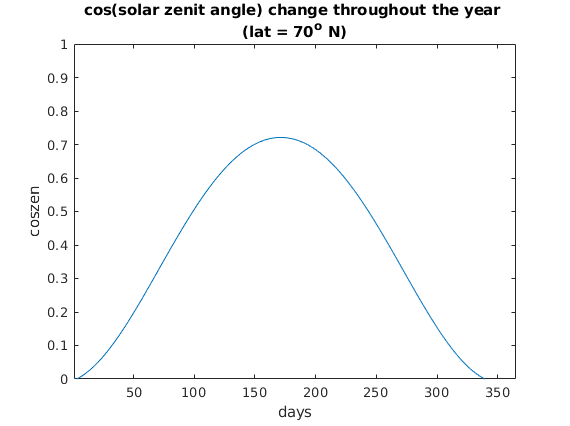
\includegraphics[width=1.1\linewidth]{coszen2.png} \\ а)}
    \end{minipage}
    \hfill
    \begin{minipage}[h]{0.49\linewidth}
        \center{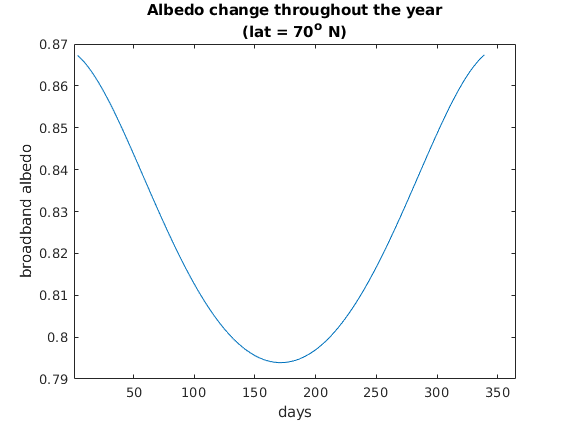
\includegraphics[width=1.1\linewidth]{coszen3.png} \\ б)}
    \end{minipage}
    \caption{Изменение (а) косинуса солнечного зенитного угла и (б) альбедо снега в течении года, вызванные вращением Земли вокруг Солнца (на примере $70\degree$ С.Ш.)}
    \label{fig:image}
\end{figure}


\subsection{Метаморфизм снега}

С течением времени после снегопада из-за изменений температуры, под действием давления снежные кристаллы изменяют свою форму от изначально близкой к сферической до очень сложных (например, фрактальная "Снежинка Коха"), а также увеличиваются в размерах, слипаясь \cite{Grenfell1999, Grenfell2005, He2018}. Это приводит к уменьшению отражающей способности заснеженной поверхности, что особенно заметно в случае длин волн, относящихся к ближнему ИК-диапазону ($0.7-5.0$ мкм). Также важным для описания метаморфизма является наличие в слое снега жидкой воды и перезамерзших кристаллов. Эти факоры играют наибольшую роль в переходные сезоны, когда происходит активное таяние или, ноборот, формирование снежного покрова.


Для описания снежных кристаллов с достаточно хорошой точностью можно использовать ледяные шарообразные частицы, сохраняющие удельную площадь поверхности ($SSA$), в том числе, в случаях кристаллов сложных форм \cite{Grenfell1999}. Их главная характеристика - эффективный радиус ($r_e$). Он определяется как средневзвешенный по площади радиус ансамбля таких частиц и связан с удельной площадью поверхности ($SSA$) и плотностью льда $\rho_{ice}$ следующим образом \cite{Flanner2006}:  
\begin{equation}
    r_e = \dfrac{3} {\rho_{ice} \cdot SSA} \label{sys}
\end{equation}
Таким образом, старение снега можно описывать как эволюцию эффективного радиуса снежного кристалла. Рассмотрим зависимость, использованную в климатической модели CLM4.5 \cite{CLM4.5tech}. Пусть момент времени $t$ соответствует текущему шагу по времени, а $(t - 1)$ - прошлому. Тогда старение снега можно описать следующим уравнением:
\begin{equation}
    r_e(t) = [r_e (t - 1) + \delta r_{e , dry} + \delta r_{e , wet} ] f_{old} + r_{e ,0} f_{new} + r_{e , rfz} f_{rfrz}, \label{sys}
\end{equation}
где $ r_{e ,0} = 54.5 $ мкм и $r_{e , rfz} = 1000 $ мкм - значения эффективного радиуса, соответствующие свежевыпавшему и перезамерзшему снегу, $\delta r_{e , dry}$ и $\delta r_{e , wet}$ - вклады в приращение от сухого и мокрого снега, $f_{old}$, $f_{new}$ и $f_{rfrz}$ - доли лежалого, свежевыпавшего и перезмерзшего снега соответственно.  

Эволюция сухого снега описывается следующим уравнением \cite{Flanner2007, CLM4.5tech}:
\begin{equation}
    \dfrac{d}{dt} \delta r_{e , dry} = {\left( \dfrac{dr_{e , dry}}{dt} \right)}_0 \left(\dfrac{\eta}{\eta + (r_e - r_{e, 0})}\right)^{1 / \kappa}, \label{sys}
\end{equation}
где ${\left( \dfrac{dr_{e , dry}}{dt} \right)}_0$, $\eta$, $\kappa$ - некоторые табличные параметры, зависящие от температуры снега, температурного градиента и плотности снега, причем для каждого значения $SSA$ они различные. Эти данные находятся в открытом доступе (\url{http://snow.engin.umich.edu/snowaging/}). Они охватывают следующие дипазоны параметров: по температуре от 223.15 до 273.15 К, по плотности от 50 до 400 кг/м$^3$, по температурному градиенту от 0 до 300 К/м для следущего набора значений $SSA$: 60, 80, 100 м$^2$/кг.

Эволюция мокрого снега описывается следующим уравнением \cite{CLM4.5tech}:
\begin{equation}
\dfrac{d}{dt} \delta r_{e , wet} = \dfrac{10^{18} C ^3} {4 \pi r_{e}^2}, \label{sys}
\end{equation}
где $C = 4.22 \cdot 10^{-13}$, $f_{liq}$ - доля жидкой воды в снегу.

Учитывая, что нас интересует суммарный вклад и от сухого, и от мокрого снега, предыдущие два уравнения можно объединить в одно. Используя в качестве начального условия для эффективного радиуса значение с прошлого шага по времени, получаем следующую задачу Коши:
\begin{equation}
    \begin{cases}
        \dfrac{d}{dt} \delta (r_{e , dry} + r_{e , wet}) = {\left( \dfrac{dr_{e , dry}}{dt} \right)}_0 \left(\dfrac{\eta}{\eta + (r_e - r_{e, 0})}\right)^{1 / \kappa} + \dfrac{10^{18} C_1 ^3} {4 \pi r_{e}^2} ,
        \\
        \delta (r_{e , dry} + r_{e , wet})(t-1) = 0
    \end{cases} \label{sys}
\end{equation}
Данное дифферненциальное уравнение предлагается решать численно.

\begin{figure}[h]
    \center{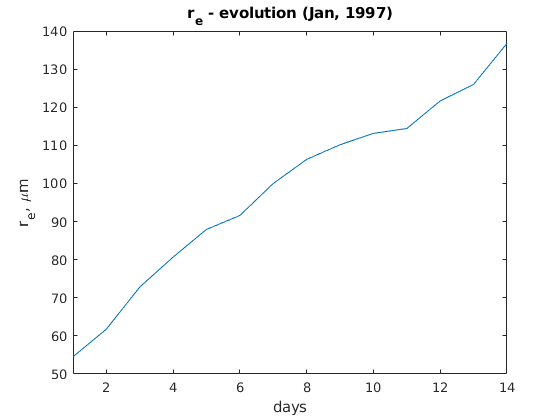
\includegraphics[scale=0.85]{rds1.png}}
    \caption{Изменение эффективного радиуса снежного кристалла за первые 2 недели января, рассчитанное по описанной выше зависимости}
    \label{fig:image}
\end{figure}
 

\subsection{Загрязнение снега атмосферными аэрозолями}

Выпадение на заснеженную поверхность атмосферных аэрозолей приводит уменьшаению ее отражающей способности. Одним из таких аэрозолей является черный углерод (ЧУ) или сажа. Основными источниками сажевого аэрозоля являются выбросы, возникающие при сжигании различных видов топлива, а также лесные и степные пожары. В качестве меры данного явления можно рассматривать концентрацию ЧУ в снегу.

Пусть имеются следующие среднемесячные климатические данные (это предположение оправдано, так как в климатических моделях данные обычно приводятся по календарным месяцам):
\begin{itemize}
    \item $H_{snw}$ - водно-эквивалентная толщина снега, 
    \item $I_{bc}$ - поток черного углерода на поверхности снежного слоя, 
    \item $Q_{melt}$ - поток талой воды на нижней границе снежного слоя,
    \item $\sigma$ - доля ячейки сетки, покрытая снегом,
    \item $F_{sw}^{down}$ – поток приходящей коротковолновой радиации
\end{itemize} 
Также дополнительно предположим, что имеет место равномерное перемешивание частиц атмосферного аэрозоля и снежных гранул.

Рассмотрим следующие промежуточные поля за n-ый месяц, необходимые для вычисления концентрации ЧУ в снегу: 
\begin{itemize}
\begin{itemize}
    \item приток массы ЧУ в ячейке, покрытой снегом:
    \begin{equation}
        P_{bc}^n = I_{bc}^n \Delta t \sigma^n S   \label{sys}
    \end{equation}
    \item масса снега в ячейке сетки:
    \begin{equation}
        M_{sn}^n = H_{snw}^n \rho_w S   \label{sys}
    \end{equation}
\end{itemize} 
\end{itemize} 
Здесь $\rho_w$ = 1000 кг/м$^3$ , $S$ – площадь ячейки сетки, $\Delta t$ = 1 месяц.
    
Массу ЧУ в заснеженной ячейке сетки $M_{bc}$ можно рассчитать на основе балансового соотношения, предложенного в работе \cite{Flanner2007}:

\begin{equation}
    \dfrac{dM_{bc}}{dt} = - C_{MSE}  Q_{melt} \dfrac{M_{bc}}{M_{sn}} S + I_{bc} \sigma S     \label{sys}
\end{equation}
Данное соотношение можно переписать в дискретном виде следующим образом:

\begin{equation}
   M_{bc}^{n+1} = M_{bc}^n - C_{MSE} Q_{melt}^{n+1} \dfrac{M_{bc}^n}{M_{sn}^n} S \Delta t + P_{bc}^{n+1}     \label{sys}
\end{equation}
Здесь $Q_{melt} = - \dfrac{1}{S} \dfrac{dM_{sn}}{dt} \geq 0$ -  средний по ячейке поток массы растаявшего снега, $C_{MSE}$ - коэффициент вымывания частиц ЧУ талой водой. Если считать, что поток ЧУ из атмосферы $I_{bc}^{n + 1} = 0$, то из прошлого уравнения следует, что:

\begin{equation}
   C_{MSE} = \dfrac{\Delta M_{bc} / M_{bc}}{\Delta M_{sn} / M_{sn}}     \label{sys}
\end{equation}
То есть коэффициент $C_{MSE}$ – это отношение вымываемой относительной массы ЧУ к относительной
массе талой воды.

В качестве начальных данных для дискретного балансового уравнения можно использовать следующее выражение:
\begin{equation}
    M_{bc}^0 = P_{bc}^0, \label{sys}
\end{equation}
где нулевой индекс означает месяц, когда в данной ячейке сетки появился снежный покров. 

Зная решение балансового уравнения за каждый месяц, можно найти концентрацию ЧУ в снегу по
следующей формуле:
\begin{equation}
   C_{bc}^n = \dfrac{M_{bc}^n}{M_{sn}^n}  \label{sys}
\end{equation}


\begin{figure}[h]
    \center{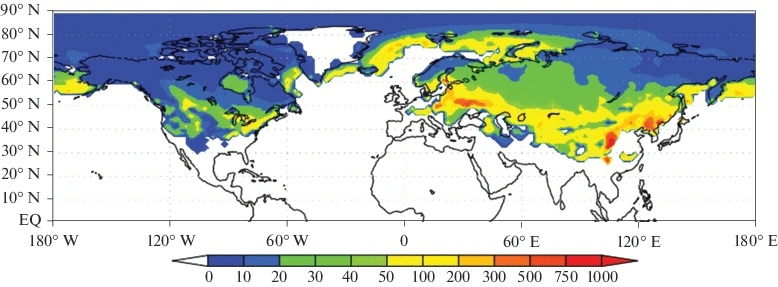
\includegraphics[scale=0.6]{Cbc1.jpg}}
    \caption{Среднемесячная концентрация черного углерода в снегу за январь 1998 год, рассчитанная по данным климатической модели ИВМ РАН, [нг/г]}
    \label{fig:image}
\end{figure}

\begin{figure}[h]
    \center{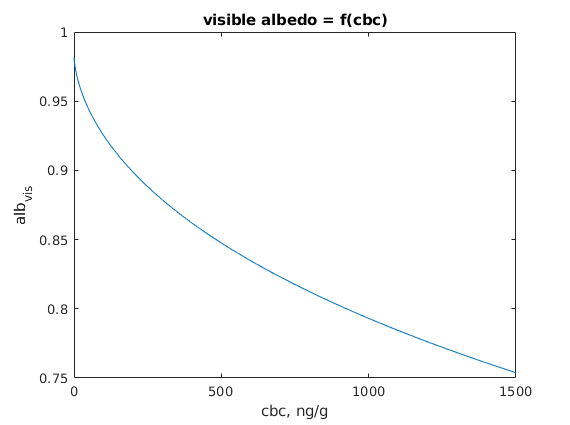
\includegraphics[scale=0.9]{alb_cbc.png}}
    \caption{Зависимость альбедо от концентрации ЧУ в снегу}
    \label{fig:image}
\end{figure}



\newpage
\section{Модификация глобальной климатической модели ИВМ РАН}

\subsection{Общие сведения о климатической модели ИВМ РАН}

Модель климата ИВМ РАН \cite{Volodin2017} состоит из атмосферного и океанического блоков. Рассматривается пятая версия модели INMCM5. Она имеет разрешение по долготе-широте $2 \times 1.5\degree$ в атмосфере и $0.5 \times 0.25\degree$ в океане. В текущей версии реализован однослойный снег. Стоит отметить, что данная версия модели участвует в международном проекте по сравнению климатических моделей CMIP6 (Coupled Models Intercomparison Project).

Нужно заметить, что в данной модели используется простая параметризация альбедо заснеженной поверхности на суше следующего вида:
\begin{equation}
    \alpha_{sn} = \begin{cases}
                        0.8,~ T \leq -1 \degree C; \\
                        0.8 - 0.1(T + 1), ~T > -1 \degree C;
                  \end{cases} \label{sys}
\end{equation}


\subsection{Описание внедренных модификаций}

Для совместного использования модели альбедо, учитывающей старение снега, и глобальной климатической модели ИВМ были необходимы следующие модификации. Во-первых, нужно было добавить в модель такую переменную, как доля жидкой воды в слое снега, а также реализовать возможность перезамерзания талой воды. Во-вторых, было необходимо добавить эволюцию плотности снега, так как ранее она считалась постоянной: $\rho_{snow} = 185.4 $ кг/м$^3$.

Определим переменные, необходимые для описания внесенных изменений: 
\begin{itemize}
    \item $S$ - водно-эквивалентная толщина слоя снега,
    \item $M_{soil}$ - вода, поступившая на поверхность почвы,
    \item $P$ - интенсивность осадков при температуре подстилающей поверхности, меньшей $0\degree $ C,
    \item $L$ - удельная теплота возгонки/сублимации, 
    \item $E$ - поток скрытого тепла на поверхность снега,
    \item $\rho_w$ - плотность воды (1 г/см$^3$),
    \item $M$ - интенсивность снеготаяния,
    \item $SW$ - талая вода, оставшаяся в слое снега,
    \item $FRZ$ - интенсивность замерзания воды, 
    \item $T_{sn}$ - температура снега, 
    \item $\Delta E$ - избыток/дефицит потока энергии в балансе тепла
\end{itemize}

В текущей версии модели водно-эквивалентная толщина слоя снега вычисляется на основании следующего уравнения баланса \cite{Volodin1998, Volodina2000}:
\begin{equation}
    \dfrac{\partial S}{\partial t} = P - M - \dfrac{E}{L} \rho_w  \label{sys}
\end{equation}
Процесс таяния начинается, когда температура подстилающей поверхности становится больше $0\degree $ C, при этом весь растаявший снег, а также возможный дождь, выпавший при наличии снежного покрова, поступают на поверхность почвы.

Идея модификации заключается в более физичном описании процесса таяния снега. Так, теперь предполагается, что при таянии снега вода не моментально уходит на верхнюю границу почвы, а постепенно просачивается сквозь толщу снега. При этом талая вода может замерзать, отдавая скрытое тепло снежному покрову. Данный процесс реализуется по следующей схеме:

Пусть $\Delta E >0$, $T_{sn} \geq 0 \degree C$ и $S^{n-1} > 0$, тогда:
\begin{equation}
    \begin{cases}
        M = \dfrac{\Delta E}{L}, \\
        S^n = S^{n-1} + P - \Delta t \left( \dfrac{E}{L} + M \right), \\
        SW_{max} = f \left( S^n \right), \\
        \Delta SW = max\{\Delta t \cdot M, SW_{max}\}, \\
        M_{soil} = max\{\Delta t \cdot M - SW_{max}, 0\}, \\
        SW^n = SW^{n-1} + \Delta SW;
    \end{cases} \label{sys}    
\end{equation}
Иначе, если  $S^{n-1} > 0$, $SW^{n-1} > 0$ и $T_{sn} \leq 0 \degree C$, то:
\begin{equation}
    \begin{cases}
        FRZ = -\dfrac{\Delta E}{L}, \\
        S^n = S^{n-1} + P - \Delta t \left( \dfrac{E}{L} - FRZ \right), \\
        SW^n = SW^{n-1} - \Delta t \cdot FRZ;
    \end{cases} \label{sys}    
\end{equation}
Критическая масса воды $SW_{max}$, способная содержаться в слое снега, определяется его пористостью $\varepsilon_{sn}$ \cite{Gusev2002}:
\begin{equation}
    M_{snwat}^{max} = M_{sn}\dfrac{\varepsilon_{sn}}{1 - \varepsilon_{sn}}  \label{sys}  
\end{equation}
Пористость снега, в свою, очередь связана с его плотностью \cite{Stock}:
\begin{equation}
    \varepsilon_{sn} = 0.11 \left( \dfrac{\rho_w}{\rho_{sn}} - 1 \right)  \label{sys}  
\end{equation}

Эволюцию плотности снега предлагается описывать аналогично тому, как это сделано в модели SWAP \cite{Gusev2002}, \cite{YOSIDA1955}:
\begin{equation}
    \rho_{sn}(\tau_i) = \rho_{sn}(\tau_{i-1}) \left[  1 + 0.1 H_{sn}(\tau_{i-1}) \exp \{ 0.08 T_{sn} - 21 \rho_{sn}(\tau_{i-1})  \} \right]    \label{sys}  
\end{equation}
В данной модели $H_{sn}$ - водно-эквивалентная толщина слоя снега в сантиметрах, плотность снега $\rho_{sn}$ вычисляется в г/см$^3$, температура слоя снега $T_{sn}$ задается в градусах Цельсия. Нужно заметить, что шаг по времени здесь $\tau_{i} - \tau_{i-1} = 1$ сутки, поэтому для использования данной зависимости в модели ИВМ необходима переинтерполяция.


\subsection{Результаты внедрения модификаций}


Для тестирования внесенных изменений в модель были проведены расчеты климата с 1997 по 2002 года с исходной и модифицированной версиями. Было установленно, что учет влагосодержания снега и реализация процесса перезамерзания талой воды приводят к тому, что снег сходит на месяц позже, а процесс формирования снежного покрова происходит более интенсивно. Так, в северном полушарии теперь в Заполярье, в горах на западном побережье Канады и Аляски, а также в районе Гималаев снег продолжает лежать до конца июня, в то время как раньше он практически весь успевал растаять в течении мая. Это хорошо согласуется с данными наблюдений за данными территориями. Вклад описанных процессов в формирование устойчивого снежного покрова в конце осени - начале зимы наиболее заметен в заполярных регионах Евразии и Гималаях. Это ожидаемо, так как процесс перезмерзания реализуется в переходные сезоны, когда температура колеблется около нулевой отметки.

Другим важным результатом внесенных изменений в модель стала возможность проводить офлайн-расчеты снежного альбедо с учетом снежного метаморфизма, так как были добавлены недостающие модельные переменные.


\newpage
\section{Модель альбедо}

В качестве примера модели альбедо можно рассматривать локально-одномерную радиационную модель SNICAR (SNow-ICe-AErosole radiation model) \cite{Flanner2007}. Данная модель описывает вертикальный перенос излучения в слое снега с заданными профилями концентраций содержащихся в нем атмосферных аэрозолей, плотности среды и размеров снежных гранул, а одним из ее выходных данных является спектральное альбедо заснеженной поверхности. Данную модель можно использовать, например, для расчета альбедо на этапе обработки данных из климатической модели. Внедрение данной модели в глобальную модель климата представляется достаточно сложной задачей. Однако, на ее основании можно построить параметризацию зависимости альбедо от основных параметров и уже ее внедрять в модель, что может позволить проводить расчеты альбедо непосредственно в процессе работы глобальной модели. 

В любом случае, используя модель SNICAR или параметризацию, построенную на ее основе, замыкая данными из модифицированной климатической модели ИВМ РАН, получаем полноценную модель альбедо.

\subsection{Построение параметризации альбедо на основе модели SNICAR}

Будем строить параметризацию альбедо от 3 переменных: эффективного радиуса снежного кристалла $r_e$, концентрации черного углерода в слое снега $C_{bc}$ и косинуса солнечного зенитного угла $coszen = cos(\theta)$ ($\theta$ - солнечный зенитный угол). Предлагается строть параметризацию в два этапа: сначала получить зависимость от $r_e$ и $C_{bc}$, а затем уточить ее за счет учета косинуса зенитного угла.

На первом этапе предлагается искать параметризацию альбедо в виде полинома от двух переменных:
\begin{equation}
    alb_1(r_e, C_{bc}) = \sum_{i,j = 0}^N \sigma_{i.j} r_e^i C_{bc}^j   \label{sys}  
\end{equation}
Данная параметризация соответствует случаю $coszen = 1$.

На втором этапе альбедо уточняется на основании эмперической зависимости \cite{Saito2019}:
\begin{equation}
    alb(r_e, C_{bc}, coszen) = \alpha + (A + B \cdot \alpha^C) \left( \dfrac{1 - coszen}{1 + coszen} \right)^D     \label{sys}  
\end{equation}
Здесь $\alpha = alb_1(r_e, C_{bc})$ - приближение с первого шага.

Параметры $\{ \sigma_{i.j} \}, A, B, C, D$ находятся на основании данных, полученных из результатов запусков модели SNICAR с различными значениями эффективного радиуса снежного кристалла, концентрации черного углерода и косинуса солнечного зенитного угла.

Полученная параметризация альбедо достаточно проста с вычислительной точки зрения, что делает возможным использование ее в глобальной климатической модели на каждом шаге по времени в будущем.


\subsection{Применение модели альбедо для вычисления радиационного форсинга, вызванного загрязнением заснеженной поверхности}

Выпадая на снег, черный углерод уменьшает альбедо поверхности,что создает дополнительный радиационный форсинг. Это может приводить к более быстрому таянию снега и повышению приземной температуры в весенний
сезон. Данный форсинг предлагается вычислять на основании изменения альбедо и данных о приходящей на поверхность радиации.

Пусть $\alpha_0$ и $\alpha_{soot}$ - альбедо чистого и загрязненного снега соответственно. Пусть $\alpha^{vis}$ и $\alpha^{nir}$ - значения альбедо для видимого ($0.3-0.7$ мкм) и ближнего ИК ($0.7-5.0$ мкм) диапазонов длин волн падающего излучения. Тогда форсинг можно оценить по следующей формуле:
\begin{equation}
    R = \sigma [ (\alpha_0^{vis} - \alpha_{soot}^{vis})F_{down}^{vis} + (\alpha_0^{nir} - \alph_{soot}^{nir})F_{down}^{nir} ] \label{sys}  
\end{equation}
Здесь $\sigma$ - доля области, покрытая снегом, а потоки радиации определяются следующим образом: $F_{down}^{vis} \approx F_{down}^{nir} \approx 0.5 \cdot F_{sw}$, где $F_{sw}$ - поток приходящей коротковолновой радиации.


%%%%%%%%%%%%%%%%%%%%%%%%%%%%%%%%%%%%%%%%%%%%%%%%%%%%%%%%%%%%%%%%%%%%%%%%%%%%%%%%%%%%%%%%%%%%%%%%%%%%%%%%%%%%%%%%%%%%%%%%%%%%%%%%%%%%%%%
\newpage
\section*{Заключение}
\addcontentsline{toc}{section}{\protect\numberline{}Заключение}






%%%%%%%%%%%%%%%%%%%%%%%%%%%%%%%%%%%%%%%%%%%%%%%%%%%%%%%%%%%%%%%%%%%%%%%%%
\newpage
\phantomsection
\addcontentsline{toc}{section}{\protect\numberline{}Список литературы}
\bibliographystyle{gost2008}
\bibliography{biblio}







\end{document} 